
%%%% CAPÍTULO 1 - INTRODUÇÃO
%%
%% Deve apresentar uma visão global da pesquisa, 
%% incluindo: breve histórico, importância e
%% justificativa da escolha do tema, delimitações
%% do assunto, formulação de hipóteses e objetivos
%% da pesquisa e estrutura do trabalho.

% Perguntas que podem guiar a introdução - não necessariamente irá ter a resposta para tudo, isso depende da área.
% 1 - Qual é o contexto em que seu trabalho está inserido?
% 2 - Qual é o problema que motiva a existência deste trabalho?
% 3 - Qual é a visão geral da literatura sobre o problema e como é tratado
% 4 - Por que a solução na literatura não é o suficiente para ?
% 5 - Como seu trabalho trata o problema ?
% 6 - como seu trabalho foi avaliado para comprovar que tratou adequadamente o problema?
% 7 - De forma geral quais foram os resultados ?
% 8 - Quais foram as contribuições do seu trabalho?
% 9 -  Como o restante da Dissertação ou Tese está organizada ?


\chapter{Introdução}\label{cap:introducao}

A alta urbanização global, em conjunto com as rápidas mudanças climáticas globais, tem intensificado a ocorrência e o impacto de desastres ambientais.
Dentre estes, alagamentos representam 40\% dos desastres e, desde o ano 2000, desastres relacionados a alagamentos têm aumentado em 134\% em comparação às décadas anteriores \cite{gar2025}.

O Brasil, em específico, pode ter impacto anual de até 50 milhões de dólares em perdas econômicas sobre infraestrutura crítica vinda de alagamentos e ciclones \cite{gar2025map}.
Em 2024, o país registrou 140 ocorrências de desastres relacionados a alagamentos, desabrigando ou desalojando 30.000 brasileiros e trazendo prejuízos públicos e privados de 47 milhões de reais \cite{addb2025}.
De acordo com análise da Defesa Civil do Rio de Janeiro, em 2019, mais de milhões de pessoas foram diretamente afetadas por inundações, alagamentos e enxurradas nas regiões da capital, metropolitana e baixada fluminense \cite{defesacivil2019}.
Em reportagem de O Globo, estima-se que as chuvas intensas no período de 2019 a 2023 causaram prejuízos de 2,9 bilhões de reais ao estado do Rio de Janeiro.

Segundo a Classificação e Codificação Brasileira de Desastres, alagamento é uma extrapolação da capacidade de escoamento de sistemas de drenagem urbana e consequente acúmulo de água em ruas,
calçadas ou outras infraestruturas urbanas, em decorrência de precipitações intensas. Esse acúmulo afeta diretamente o trânsito de veículos e pedestres, principalmente em áreas urbanas,
tornando imprescindível a vigilância de áreas possivelmente afetadas por alagamentos.

Parte da insuficiência do sistema de drenagem urbana do Rio de Janeiro vem do fato de que foi construído em grande parte no início do século XX,
não sendo projetado para suportar os volumes de precipitação atualmente registrados, intensificados pelas mudanças climáticas e pela expansão urbana não planejada \cite{planodiretor}.
Essa insuficiência estrutural, aliada à falta de manutenção periódica, como desassoreamento de canais e limpeza de galerias pluviais, compromete a capacidade de escoamento das águas pluviais.

Diante deste panorama, fica claro que a mitigação dos impactos dos alagamentos no estado do Rio de Janeiro exige não apenas intervenções estruturais,
como melhorias no sistema de drenagem e planejamento urbano, mas também o desenvolvimento de ferramentas tecnológicas que permitam a detecção precoce, monitoramento eficiente e resposta rápida a esses eventos.

\section{Contexto do problema}

Para os órgãos governamentais responsáveis pelo monitoramento de áreas urbanas, como o \acrfull{cor}, a observação constante dessas áreas urbanas é crucial para a emissão de alertas precoces e respostas eficazes.
A detecção e avaliação oportuna dos riscos de inundação permitem que as autoridades implementem planos de evacuação, desloquem serviços de emergência e iniciem medidas de controle de inundação para minimizar danos e proteger vidas.

Atualmente, o monitoramento pelo \acrshort{cor} é realizado na própria sala de controle, onde dezenas de funcionários monitoram uma quantidade ainda maior de telas que exibem as milhares de câmeras da cidade do Rio de Janeiro, como pode ser visto na Figura \ref{fig:cor}, tornando isto um trabalho árduo.

O monitoramento atualmente realizado pelo \acrshort{cor} não é automatizado. Este monitoramento não só é dependente da mão-de-obra dos funcionários frente a diversas telas, como também depende em parte de notificações enviadas por terceiros, utilizando o aplicativo do \acrshort{cor} para reportar problemas na cidade de forma direta.

\begin{figure}[htb]
\centerline{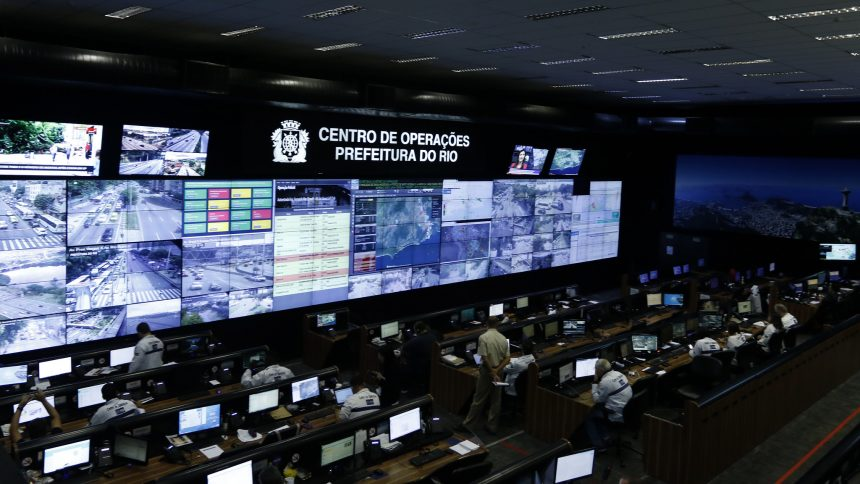
\includegraphics[width=0.9\linewidth]{images/46627458084_451cf87027_k.jpg}}
\caption{Sala central do Centro de Operações do Rio}
\label{fig:cor}
\end{figure}

\section{Objetivo}

Com base em diversas pesquisas sobre o problema das inundações urbanas utilizando diferentes Redes Neurais Convolucionais (CNN, do inglês \acrlong{cnn}),
apresentadas na Seção \ref{sec:trabalhos_alagamento},
a presente dissertação visa desenvolver uma abordagem inicial utilizando \acrshort{cnn}s com aprendizado por transferência (\textit{transfer learning}), treinadas em um conjunto de dados original,
para não apenas facilitar o monitoramento e classificação das milhares de câmeras na cidade do Rio de Janeiro pelo \acrshort{cor}.

Portanto, esta pesquisa foi estruturada em quatro etapas principais: (i) aquisição e preparação dos dados, (ii) seleção das arquiteturas de redes neurais, (iii) treinamento e validação dos modelos, e (iv) avaliação do desempenho e análise dos resultados.

Os dados foram obtidos por meio de câmeras do \acrshort{cor}, enquanto a escolha das arquiteturas foi embasada em uma revisão criteriosa da literatura referente ao reconhecimento e classificação de alagamentos.

O treinamento e a validação foram conduzidos inicialmente por meio de validação simples, com o intuito de identificar o modelo de melhor desempenho. Posteriormente, esse modelo selecionado foi submetido a uma validação cruzada, proporcionando uma avaliação mais robusta e confiável dos seus resultados.

Finalmente, o desempenho do modelo foi comparado com resultados obtidos em outros conjuntos de dados, visando avaliar sua capacidade de generalização.

A seção seguinte apresenta uma descrição dos capítulos que abordam cada uma dessas etapas de forma aprofundada.

%Todos os modelos foram treinados em conjunto de dados original formado por imagens do circuito de câmeras do Centro de Operações do Rio.
%Todas as câmeras neste conjunto de dados são fixas, de forma que não há nenhuma modificação na paisagem ao longo do dia.

\section{Organização do Texto}\label{Organização do texto}

O capítulo \ref{cap:fundamentação} explica brevemente os conceitos mais importantes para o desenvolvimento deste trabalho, começando por técnicas de processamento de imagem e finalizando na abordagem dos fundamentos de redes neurais.

O capítulo \ref{cap:trabalhos} considera alguns trabalhos relevantes para o problema de classificação do estado de alagamento em regiões urbanas nos últimos 5 anos.
Ao final, algumas características das tecnologias utilizadas em cada artigo, assim como as deste trabalho, são comparadas em uma tabela.

O capítulo \ref{cap:metodologia} descreve a metodologia usada na execução deste trabalho,
explicando a criação do conjunto de dados, a escolha das arquiteturas de \acrshort{cnn}s inicialmente empregadas e as métricas utilizadas para a comparação dos resultados.

O capítulo \ref{cap:resultados} apresenta e discute os resultados do treinamento das diferentes arquiteturas comparadas.
O modelo com melhor performance é mais detalhadamente avaliado após a inclusão de alterações no pré-processamento e uso de diferentes conjuntos de dados de entrada.

O capítulo \ref{cap:conclusoes} sumariza as contribuições e limitações deste trabalho, apresentando conclusões relacionadas aos seus resultados.
Também discute possíveis pontos para melhorias futuras em prosseguimentos da linha de pesquisa.

No Apêndice \ref{apendA} estão citadas os códigos das câmeras do COR usadas e os números de imagens de cada classe delas armazenadas no conjuntos de dados inicial da pesquisa.

\section{Contribuições e legados concretos desta dissertação}\label{Contribuições}

Até o momento com os resultados deste trabalho foram publicados no IEEE \cite{goncalves2024} contribuindo, também, com a disponibilização dos três conjuntos de dados (treino, validação e teste)
correspondentes a organização que se fez nas diversas etapas desta dissertação e os programas de computador (fontes e executáveis) desenvolvidos. 
Esses se encontram publicamente disponíveis em \href{https://doi.org/10.5281/zenodo.15670835}{10.5281/zenodo.15670835}.